\documentclass[tikz]{standalone}

\usepackage{amssymb}
\usetikzlibrary{calc}
\usetikzlibrary{decorations.markings}
\begin{document}
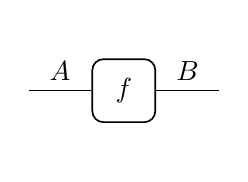
\begin{tikzpicture}[unit length/.code={{\newdimen\tikzunit}\setlength{\tikzunit}{#1}},unit length=4mm,x=\tikzunit,y=\tikzunit,semithick,outer box/.style={draw=none},box/.style={rectangle,draw,solid,rounded corners},circular box/.style={circle,draw,solid},junction/.style={circle,draw,fill,inner sep=0},variant junction/.style={circle,draw,solid,inner sep=0},invisible/.style={draw=none,inner sep=0},wire/.style={draw,postaction={decorate},decoration={markings,mark=at position 0.5 with {\node[anchor=south] {#1};}}}]
\node[outer box,minimum width=6\tikzunit,minimum height=4\tikzunit] (root) at (0,0) {};\node[box,minimum size=2\tikzunit] (n3) at (0,0) {$f$};\path[wire=$A$] (root.west) to[out=0,in=-180] (n3.west);\path[wire=$B$] (n3.east) to[out=0,in=180] (root.east);
\end{tikzpicture}
\end{document}
